\documentclass[justified]{tufte-handout}
\usepackage{../braph2_tut}
%\geometry{showframe} % display margins for debugging page layout

\title{Pipeline for Comparison of Connectivity Multiplex Data using Binary Weighted Undirected graphs}

\begin{document}

\maketitle

\begin{abstract}
\noindent
This tutorial is not ready. You can find a similar one in CON BUT (\url{https://github.com/softmatterlab/BRAPH-2-Matlab/blob/develop/tutorials/pipelines/tut_a_con_but/tut_a_con_but.pdf}).
\end{abstract}
\fig{marginfigure}
	{fig:01}
	{
	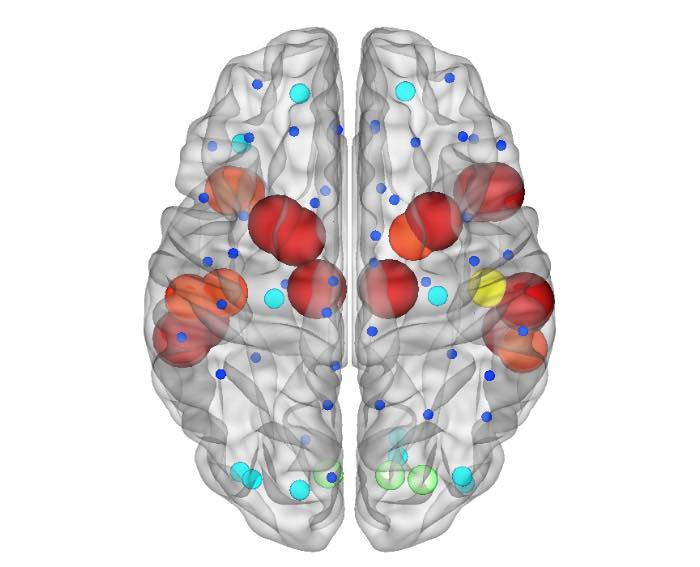
\includegraphics{fig01_01.jpg}
	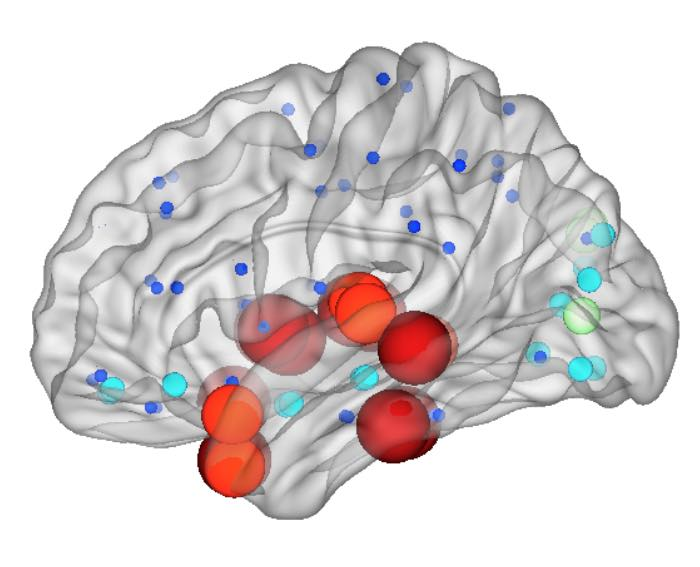
\includegraphics{fig01_02.jpg}
	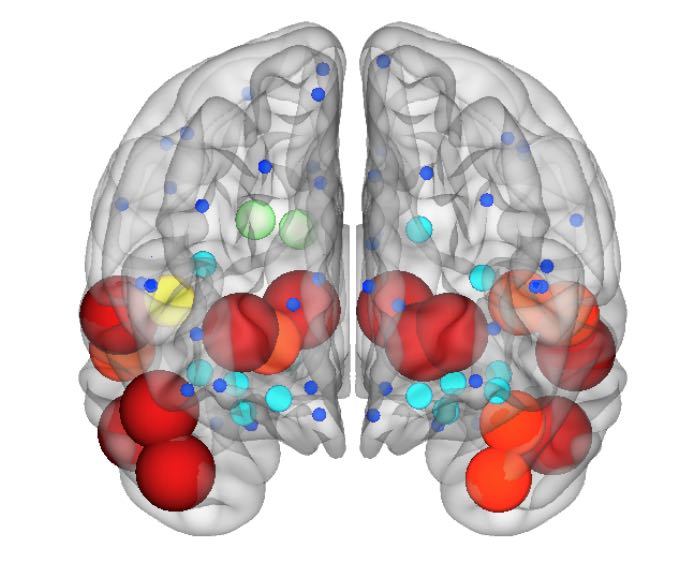
\includegraphics{fig01_03.jpg}
	}
	{Figure examples}
	{
	Examples of displays of \fn{Community Structure} with connectivity data binarized at fixed thresholds obtained using BRAPH 2.
	}
	
\tableofcontents

\clearpage
\section{Generate Example Data}

You can generate the example data by typing in the command line the instruction in \Coderef{cd:generate}.
%
\begin{lstlisting}[
	label=cd:generate,
	caption={
		{\bf Command to generate example data.}
		Command to generate the example data for connectivity and functional multiplex analyses. They will be placed in the folder \fn{./braph2/pipelines/connectivity-functional multiplex/Example data CON\_FUN\_MP XLS}, and include the brain atlas \fn{atlas.xlsx}, two folders (one for the connectivity data and the other for the functional data) with two folders with the subject files (\fn{CON\_Group1\_XLS} and \fn{CON\_Group2\_XLS} for the connectivity data, and \fn{FUN\_Group1\_XLS} and \fn{FUN\_Group2\_XLS} for the functional data), and the associated covariates files (\fn{CON\_Group1\_XLS.vois} and \fn{CON\_Group2\_XLS.vois} at the connectivity data, and \fn{FUN\_Group1\_XLS.vois} and \fn{FUN\_Group2\_XLS.vois} at the functional data). The details about the format of these files can be found in the tutorials \href{https://github.com/braph-software/BRAPH-2/tree/develop/tutorials/general/tut_ba}{Brain Atlas}, \href{https://github.com/braph-software/BRAPH-2/tree/develop/tutorials/general/tut_gr_con_fun_mp}{Group of Subjects with Connectivity-Functional Multiplex Data}.
	}
]
test_CombineGroups_CON_FUN_MP
\end{lstlisting}

\section{Open the GUI}

The general GUI of BRAPH 2.0 can be opened by typing \code{braph2} in MatLab's terminal. This GUI allows you to select a pipeline, in this case, \emph{Pipeline Connectivity-Functional Multiplex Comparison WU}, as shown in \Figref{fig:02}.

\fig{figure}
	{fig:02}
	{
	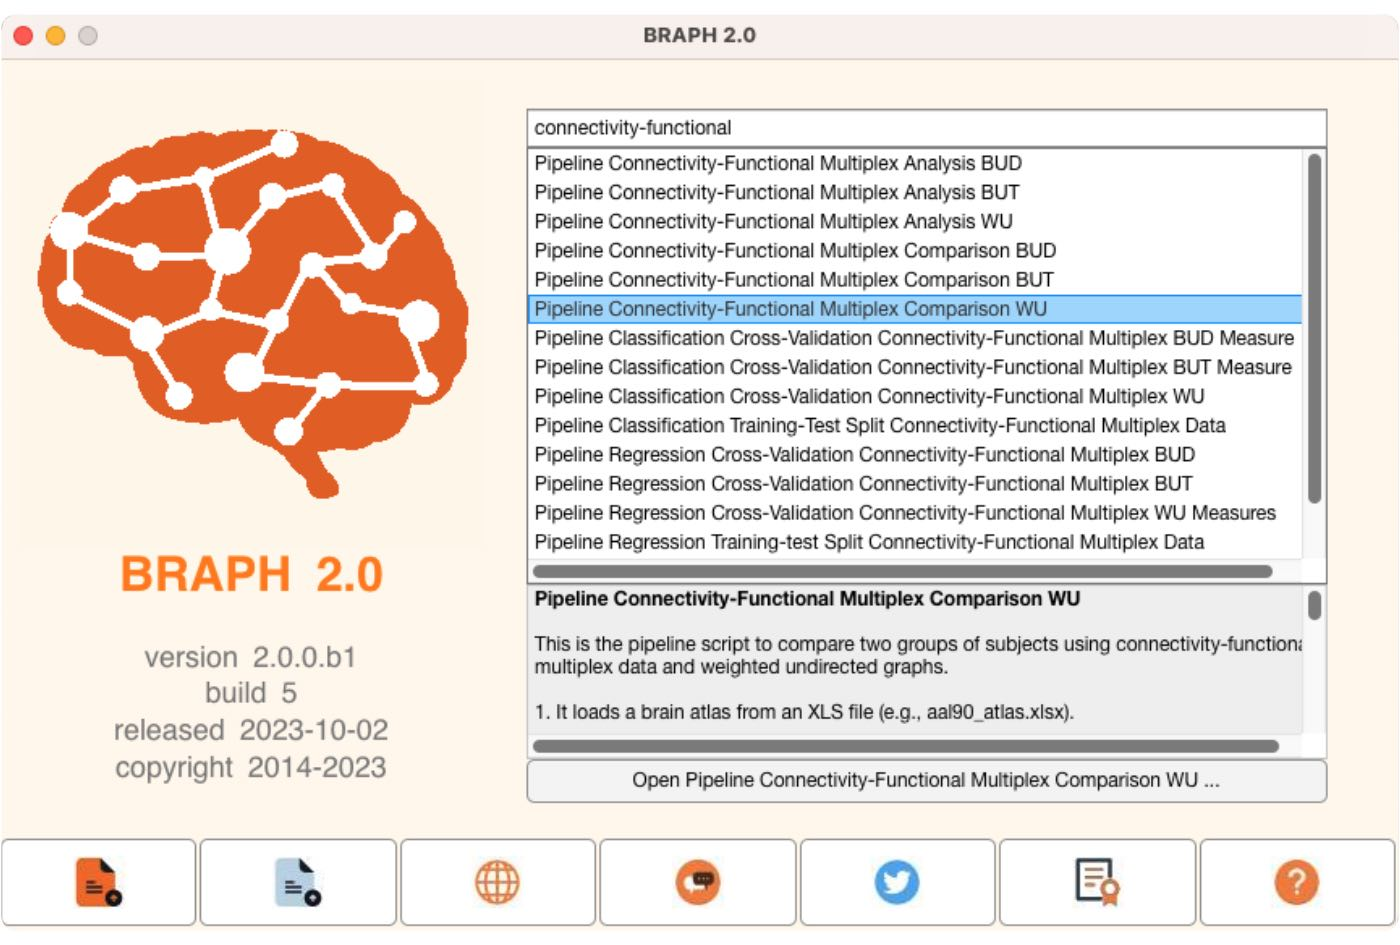
\includegraphics{fig02.jpg}
	}
	{BRAPH 2 main GUI}
	{
	BRAPH 2 main GUI with the pipeline \emph{Pipeline Connectivity-Functional Multiplex Comparison WU} selected.
	}

\begin{tcolorbox}[
	title=Pipeline launch from command line
]
To open the GUI and upload the connectivity-functional multiplex comparison pipeline, you can also do it from the command line by typing the commands in \Coderef{cd:launch}.
%
\begin{lstlisting}[
	label=cd:launch,
	caption={
		{\bf Code to launch the GUI to upload a pipeline file to compare two groups of subjects.}
		This code can be used in the MatLab command line to launch the GUI to upload a pipeline file.
	}
]
im = ImporterPipelineBRAPH2( ...
	'FILE', which('pipeline_connectivity_functional_multiplex_comparison_wu.braph2') ...
	);
pip = im.get('PIP');

gui = GUIElement('PE', pip, 'WAITBAR', true); gui.get('DRAW')
gui.get('SHOW')
\end{lstlisting}
\end{tcolorbox}

Once the pipeline is uploaded, you can see a GUI that contains different steps to: upload a brain atlas, upload the connectivity and functional multiplex data of two groups, analyze them, and finally, compare the groups (\Figref{fig:03}). 

\fig{marginfigure}
	{fig:03}
	{
	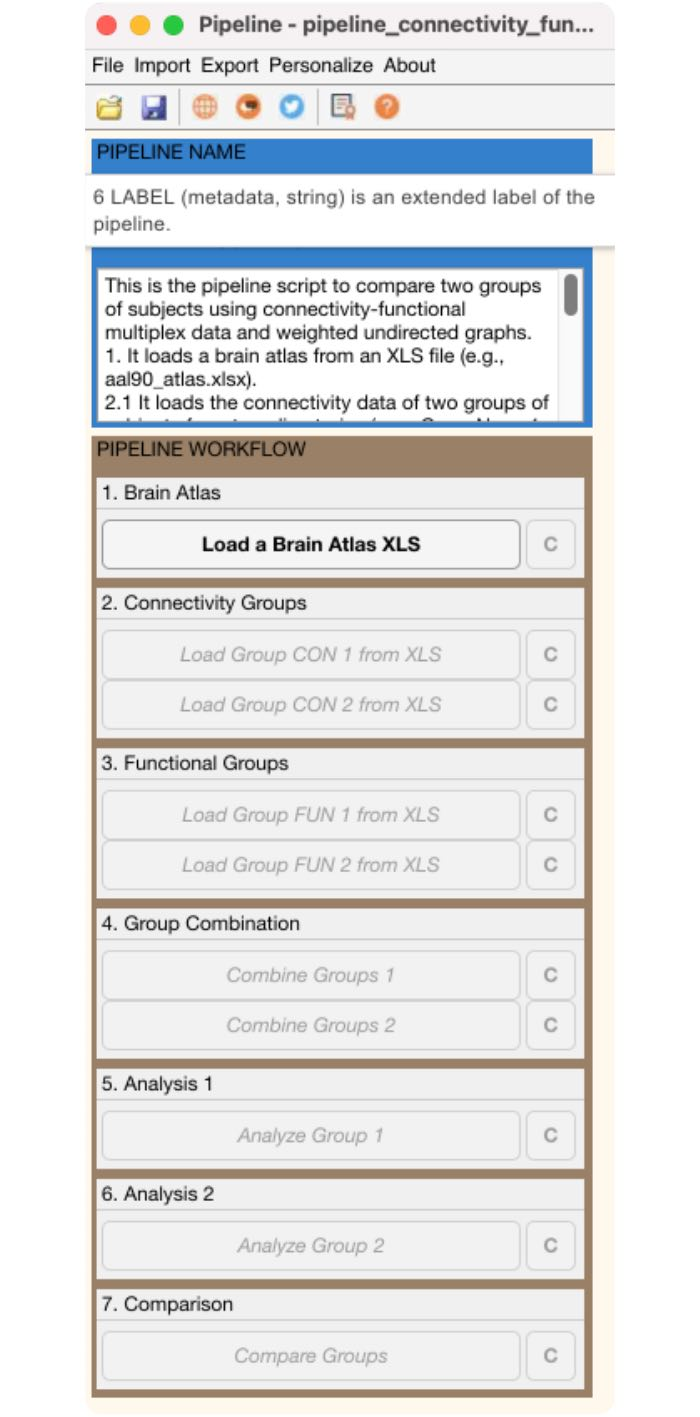
\includegraphics{fig03.jpg}
	}
	{Pipeline steps}
	{
	These are the steps of the pipeline. Only the first step is active when the pipeline is first opened. Subsequent steps will become active sequentially.
	}

\clearpage
\section{Step 1: Load the Brain Atlas}

\Figref{fig:04} shows how to upload and plot the brain atlas that you used to extract the \emph{connectivity-functional multiplex data} for your analysis. For more information on where to find different atlases or how to change plotting settings on the brain surface, check the tutorial \href{https://github.com/braph-software/BRAPH-2/tree/develop/tutorials/general/tut_ba}{Brain Atlas}.

\fig{figure*}
	{fig:04}
	{
	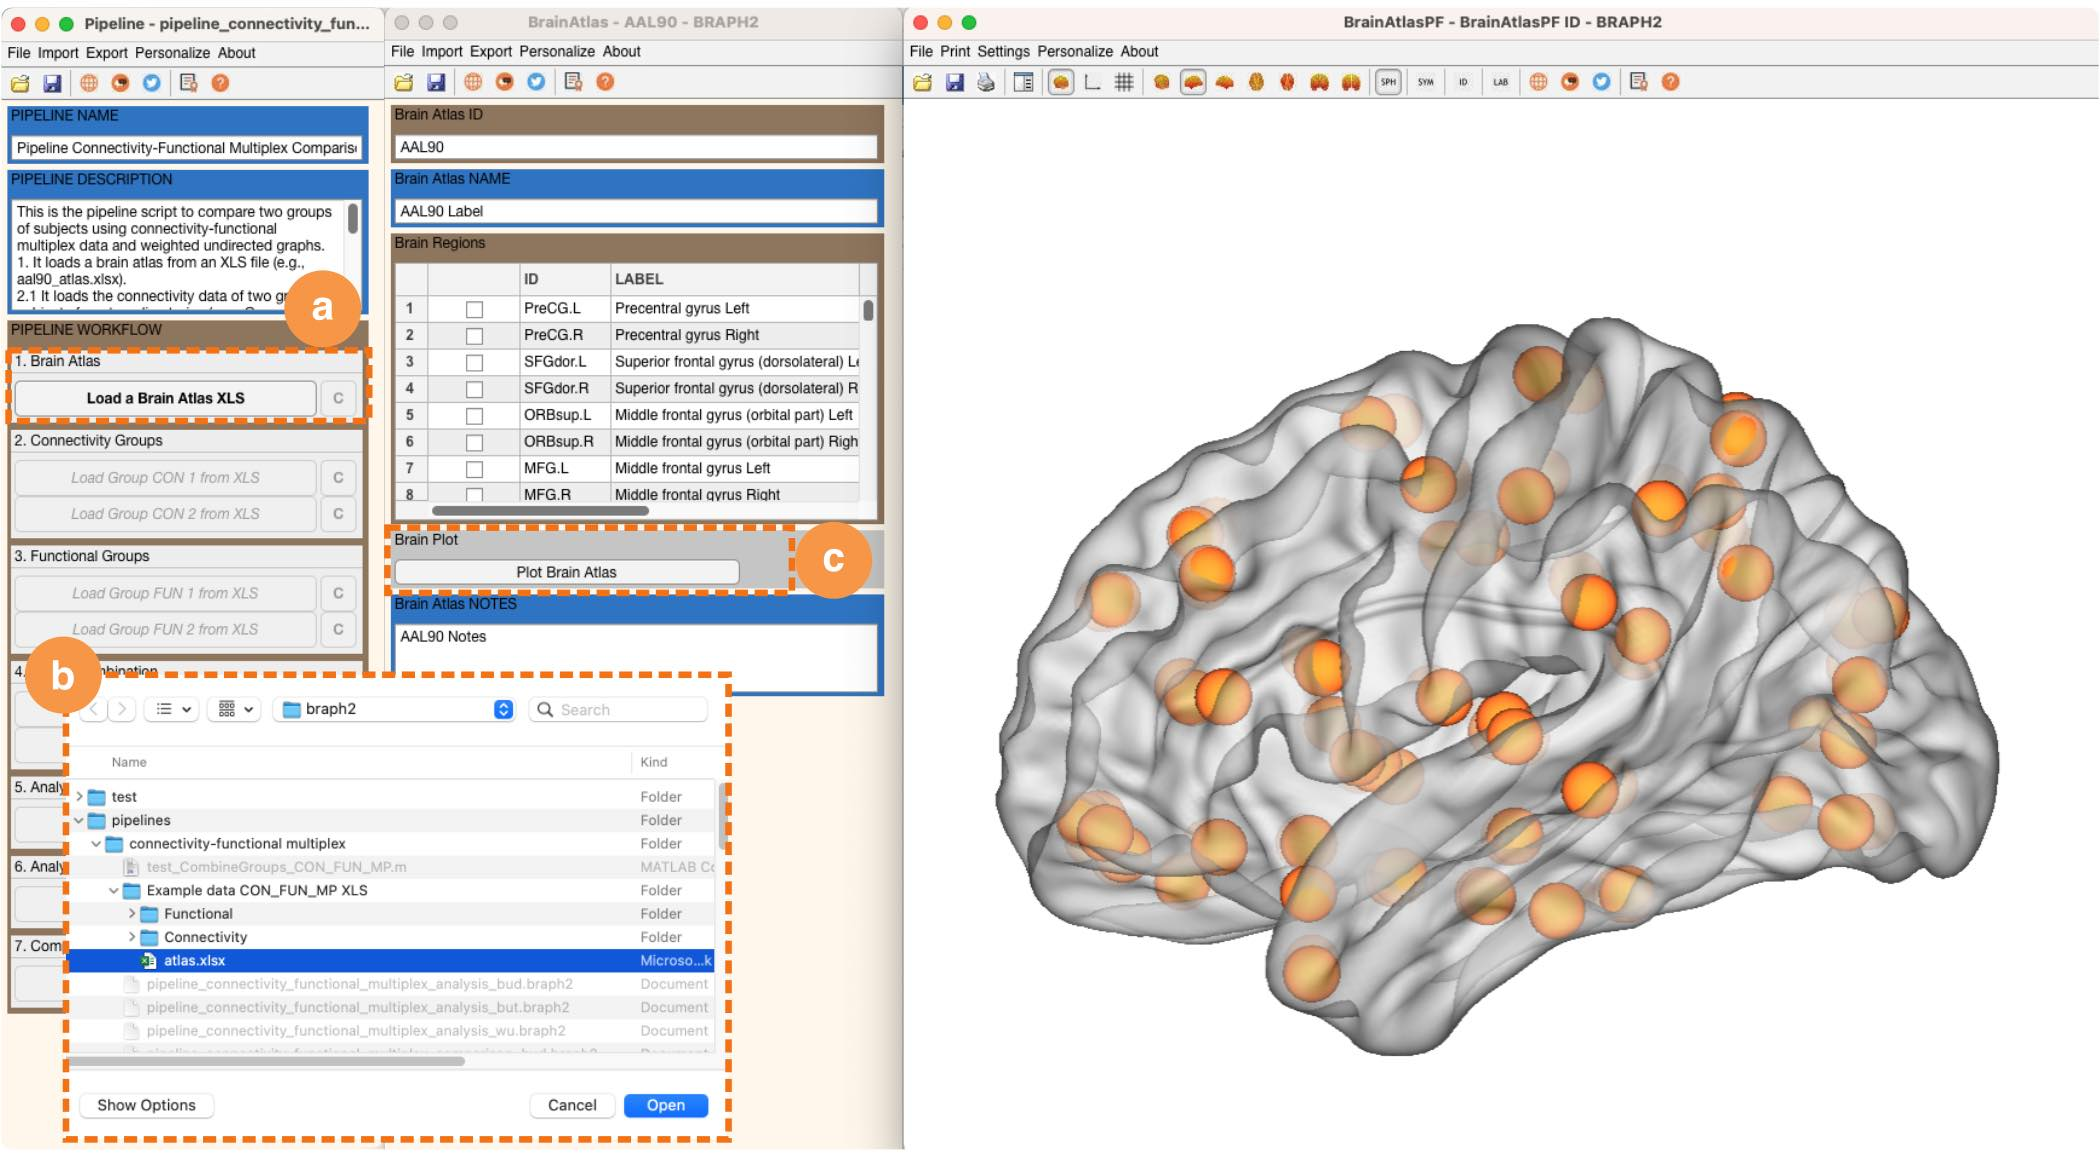
\includegraphics{fig04.jpg}
	}
	{Uploading the Brain Atlas}
	{
	Steps to upload the brain atlas:
	{\bf a} Click on \fn{Load Atlas} from the pipeline GUI.
	{\bf b} Navigate to the BRAPH~2.0 folder \fn{pipelines\_connectivity-functional multiplex\_Example data CON\_FUN\_MP XLS}, and select the atlas file, in this example the \fn{atlas.xlsx}.  
	{\bf c} You can visualize the brain atlas by pressing \fn{Plot Brain Atlas}. 
	}
 
\clearpage
\section{Step 2: Load the Connectivity-Functional Multiplex Group Data}

After you loaded the brain atlas, you can upload the \emph{connectivity data} for each group and later the \emph{functional data} for each group, as shown in \Figref{fig:05}. A new interface will be shown containing the data for the group you just selected. You can open each subject’s data by selecting the subject, right click, and select “Open selection” (for more information check the tutorial \href{https://github.com/braph-software/BRAPH-2/tree/develop/tutorials/general/tut_gr_con_fun_mp}{Group of Subjects with Connectivity-Functional Multiplex Data}).

\fig{figure*}
	{fig:05}
	{
	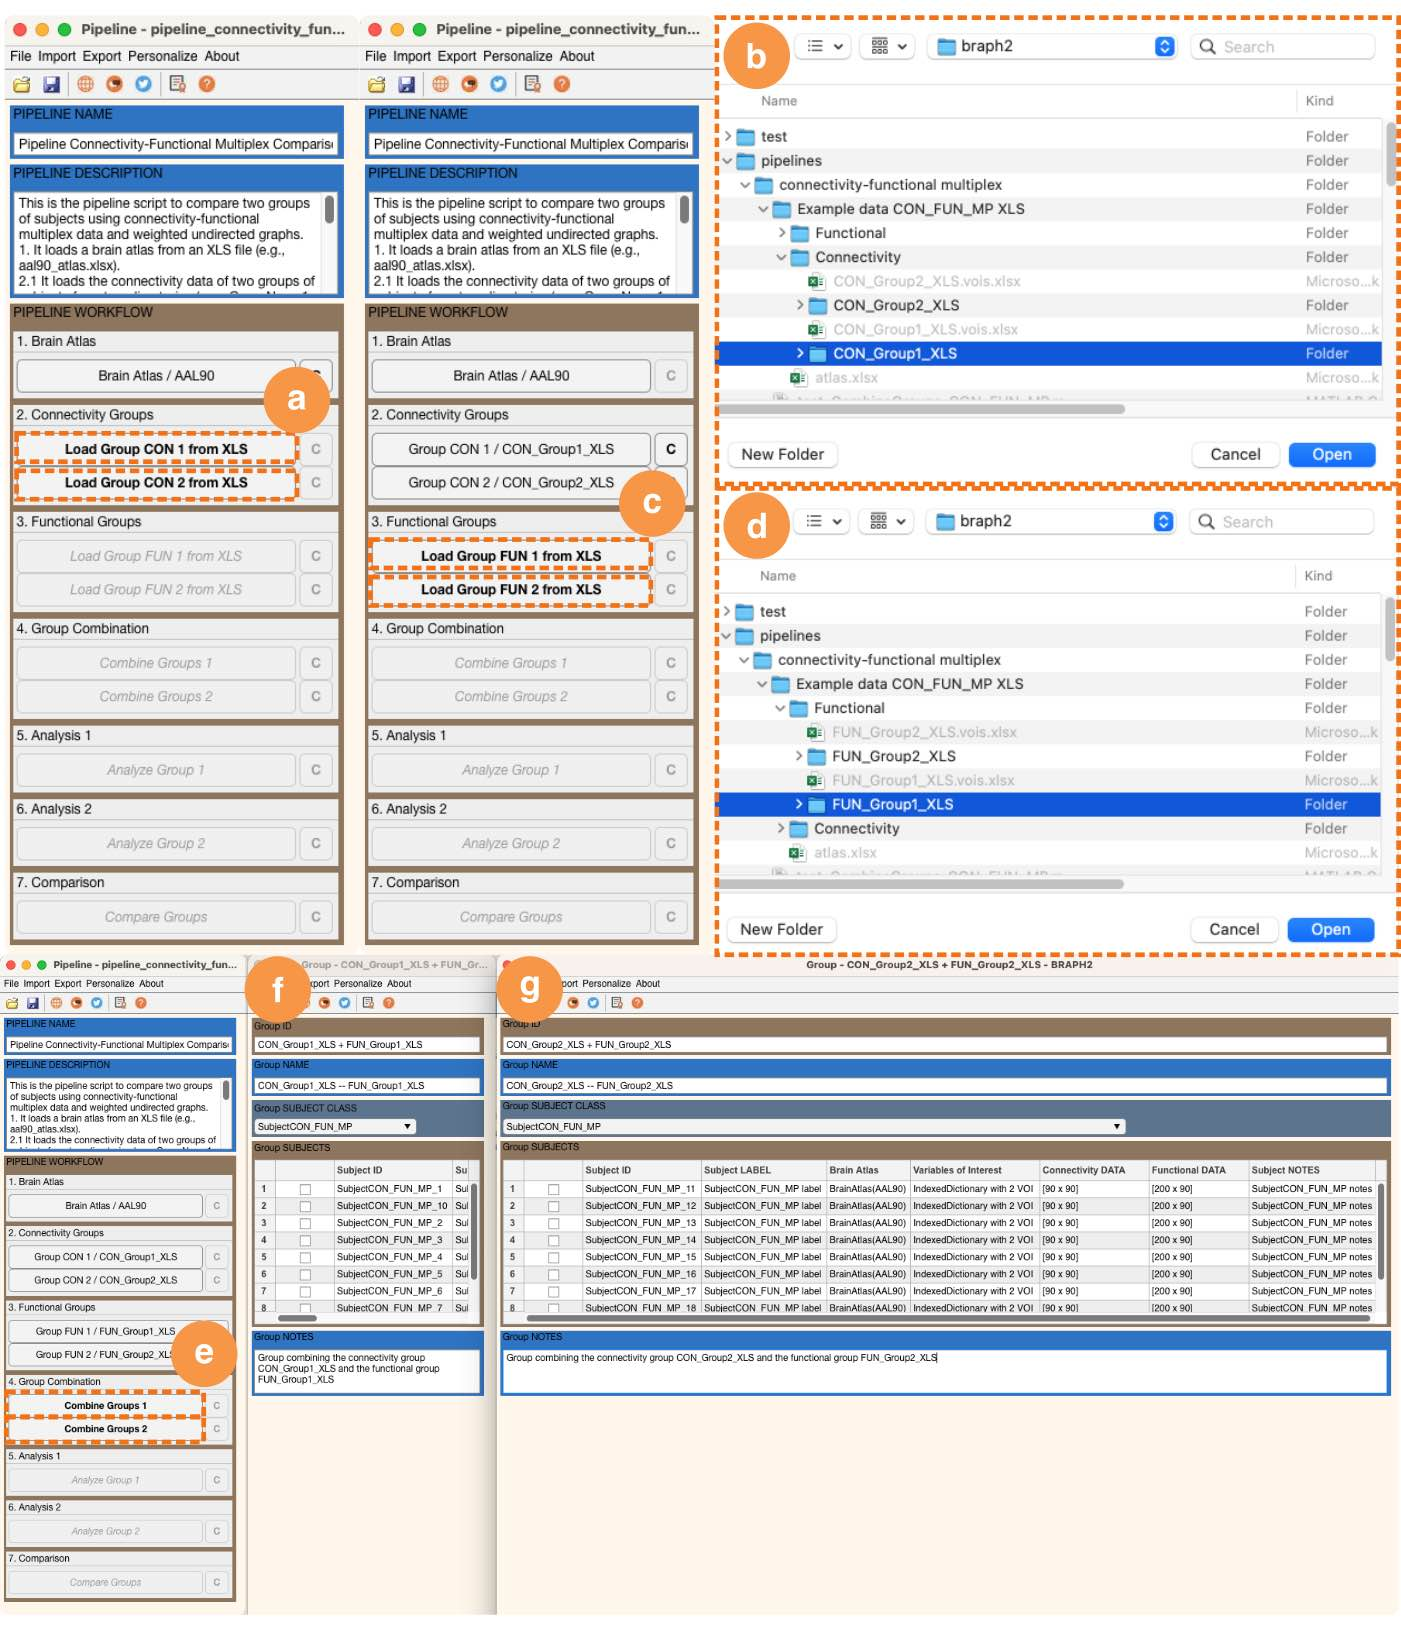
\includegraphics{fig05.jpg}
	}
	{Loading and visualizing the group data}
	{
	{\bf a} From the pipeline GUI, click on \fn{Load Group CON 1 from XLS} to load the data of group 1.
	{\bf b} Once the data is uploaded, you can select a subject, right click and select \code{Open selection}.
	{\bf c} This will open the connectivity matrix of the subject in addition to the age and sex of that subject (which are the variables of interest available for the example data).
	You can then repeat the same procedure for group 2.
	}
\end{document}